\lstset{
 upquote=true,
 showspaces=false,
 showtabs=false,
 frame=none,
 tabsize=2,
 breaklines=true,
 numbers=none,
 showstringspaces=false,
 breakatwhitespace=true,
 escapeinside={(*@}{@*)},
 keywordstyle=\bfseries,
 basicstyle=\footnotesize\ttfamily,
}






\section*{Lab activity 3}
\subsection*{Topology diagram}
\begin{figure}[htb]
	\centering
	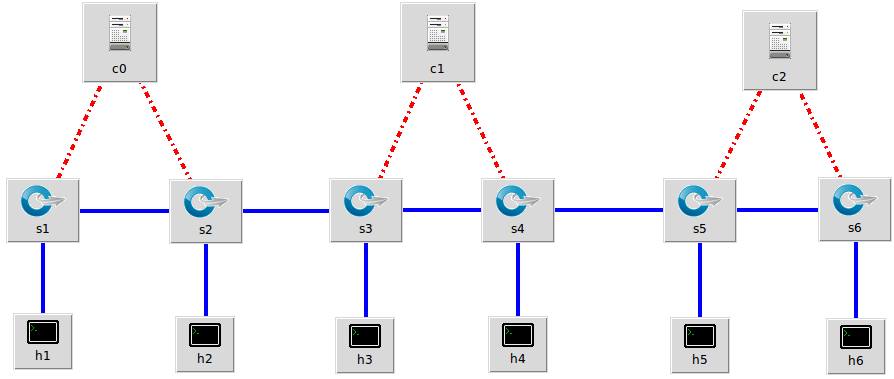
\includegraphics[width=1\linewidth]{img/topology-3.png}
	\caption{the simple linear topology that will be implemented in this activity. It is
  assumed that c1 and c2 are remote controllers running on the same machine
  on which Mininet is running, respectively on the TCP ports 6634 and 6635,
  while c0 is a local controller.}
	\label{fig:topology-3}
\end{figure}







\subsection*{Learning objectives}
After finishing this lab activity you will be able to:
\begin{itemize}
  \item Use the tool ovs-vsctl for implementing a cluster of controllers inside Mininet
  \item Test the network connectivity and the performance of a network with multiple
  controllers
  \item Dynamically set the controller for any switch of a generic running Mininet
  network using the tool ovs-vsctl.
\end{itemize}






\subsection*{Scenario}
In this activity you will implement the topology shown in figure \ref{fig:topology-3}
using the command \code{mn} to create and start a new Mininet network, passing
\code{--topo} as parameter to specify the required topology. You will then
use the tool ovs-vsctl in order to set the controller for each switch according
to the topology diagram shown in figure \ref{fig:topology-3}.

Begin by creating and starting a new Mininet network using the command \code{mn}.
Once the network is running, start the remote controllers and use the tool ovs-vsctl
for setting the controller for each switch according to the topology diagram.
To conclude, test the network verifying the connectivity between all hosts.

This lab activity assumes that:
\begin{itemize}
  \item you are proficient in SDN networks
  \item you are proficient in Mininet network emulator
  \item you have already completed the previous lab activities of this paper.
\end{itemize}






\subsection*{Task 1: create and start the network}
Create and start a new Mininet network, using the parameter \code{--topo} to
specify the required topology:
\begin{lstlisting}
$ sudo mn --topo linear,6
\end{lstlisting}
After executing this command the network will be running and a single local controller
(called \code{c0}) will be used for all the switches.


\subsection*{Task 2: start the remote controllers}
\subsubsection*{Step 1}
Open a new terminal and move to the directory \code{/home/mininet/pox}

\subsubsection*{Step 2}
Start the first POX controller, using the component \code{forwarding.l2\_learning}
for making the OpenFlow switches act as L2 learning switches and the component
\code{openflow.of\_01} for specifying the TCP port to listen for connections on.

\lstset{basicstyle=\scriptsize\ttfamily}
\begin{lstlisting}
$ sudo ./pox.py forwarding.l2_learning openflow.of_01 --port=6634
\end{lstlisting}

\subsubsection*{Step 3}
Open a new terminal and repeat step 1 and step 2 for starting the second controller.
Remember to specify the correct TCP port, which this time will be 6635 instead of 6634.




\subsection*{Task 3: set the controller for each switch}
\subsubsection*{Step 1}
Open a new terminal and use ovs-vsctl to connect the switch \code{s3} to the POX
controller listening on port 6634 \cite{ref-8}:
\begin{lstlisting}
$ sudo ovs-vsctl set-controller s3 tcp:127.0.0.1:6634
\end{lstlisting}
On the terminal with which you started that controller you should see that a new
switch has connected, like in the screenshoot below:
\begin{figure}[htb]
	\centering
	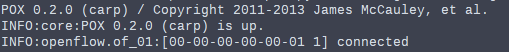
\includegraphics[width=1\linewidth]{img/controller-connection.png}
\end{figure}


\subsubsection*{Step 2}
Use ovs-vsctl to connect the switch \code{s4} to the POX controller listening on
port 6634:
\begin{lstlisting}
$ sudo ovs-vsctl set-controller s4 tcp:127.0.0.1:6634
\end{lstlisting}
Again, on the controller's terminal you should se that the switch has connected
to the controller.


\subsubsection*{Step 3}
Apply the same proceeding showed in the first two step to connect the switches
\code{s5} and \code{s6} to the POX controller listening on port 6635.



\subsection*{Task 4: test the network}
Test the connectivity between all hosts.
